%قبل از شروع مسئله ترجیحاً چیزی ننویسید. اما اگر خواستید بنویسید، در قالب لیستی (فقرات و شمارش) بنویسید.
%برای اضافه کردن نمره، بعدی از شروع‌مسئله، [x] را اضافه کنید و به جای x  نمره مورد نظر را قرار دهید. برای زیرمسئله‌ها هم به همین صورت است.
%\شروع‌مسئله[10]
\شروع‌مسئله
% صورت اصلی مسئله را در این‌جا بنویسید.
فرض کنید یک دایره به $n$ قطاع برابر تقسیم شده و روی هر کدام از قطاع‌ها یک عدد صحیح نوشته‌شده.
می‌خوایم تعدادی قطاع انتخاب کنیم به طوری که فاصله‌های آن‌ها از هم برابر باشد (مثلاً در دایره با تعداد زوج قطاع یکی در میان انتخاب کنیم) و جمع اعداد روی قطاع‌های انتخاب شده حداکثر شود. به عنوان مثال در دو شکل زیر قطاع‌های انتخاب شده برای حداکثر کردن جمع، مشخص شده‌اند.

 
 
 \tikzset{every picture/.style={line width=0.75pt}} %set default line width to 0.75pt        
 \begin{center}


\tikzset{every picture/.style={line width=0.75pt}} %set default line width to 0.75pt        

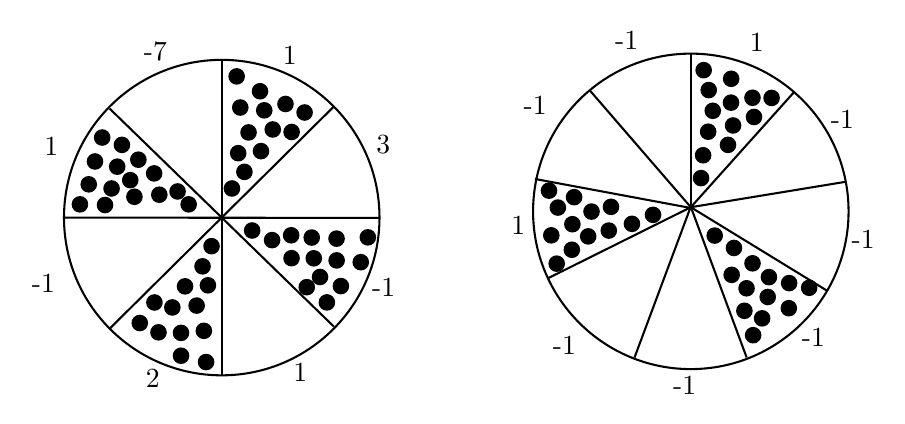
\begin{tikzpicture}[x=0.75pt,y=0.75pt,yscale=-1,xscale=1]
	%uncomment if require: \path (0,300); %set diagram left start at 0, and has height of 300
	
	%Shape: Circle [id:dp5986740273022819] 
	\draw   (151,145) .. controls (151,103.03) and (185.03,69) .. (227,69) .. controls (268.97,69) and (303,103.03) .. (303,145) .. controls (303,186.97) and (268.97,221) .. (227,221) .. controls (185.03,221) and (151,186.97) .. (151,145) -- cycle ;
	%Straight Lines [id:da6475893816865963] 
	\draw    (173,92.5) -- (281,197.5) ;
	%Straight Lines [id:da34038750959479913] 
	\draw    (281,91.5) -- (173,198.5) ;
	%Straight Lines [id:da6044840923899626] 
	\draw    (227,69) -- (227,221) ;
	%Straight Lines [id:da9151150459815314] 
	\draw    (303.03,145.15) -- (151,145) ;
	%Shape: Free Drawing [id:dp6645888691852918] 
	\draw  [color={rgb, 255:red, 0; green, 0; blue, 0 }  ,draw opacity=1 ][line width=6] [line join = round][line cap = round] (162.92,128.97) .. controls (162.92,128.97) and (162.92,128.97) .. (162.92,128.97) ;
	%Shape: Free Drawing [id:dp8198960384622548] 
	\draw  [color={rgb, 255:red, 0; green, 0; blue, 0 }  ,draw opacity=1 ][line width=6] [line join = round][line cap = round] (165.92,117.97) .. controls (165.92,117.97) and (165.92,117.97) .. (165.92,117.97) ;
	%Shape: Free Drawing [id:dp2632623334763411] 
	\draw  [color={rgb, 255:red, 0; green, 0; blue, 0 }  ,draw opacity=1 ][line width=6] [line join = round][line cap = round] (182.92,126.97) .. controls (182.92,126.97) and (182.92,126.97) .. (182.92,126.97) ;
	%Shape: Free Drawing [id:dp5492895648111484] 
	\draw  [color={rgb, 255:red, 0; green, 0; blue, 0 }  ,draw opacity=1 ][line width=6] [line join = round][line cap = round] (196.92,133.97) .. controls (196.92,133.97) and (196.92,133.97) .. (196.92,133.97) ;
	%Shape: Free Drawing [id:dp5434578693670231] 
	\draw  [color={rgb, 255:red, 0; green, 0; blue, 0 }  ,draw opacity=1 ][line width=6] [line join = round][line cap = round] (178.92,109.97) .. controls (178.92,109.97) and (178.92,109.97) .. (178.92,109.97) ;
	%Shape: Free Drawing [id:dp6282637486931193] 
	\draw  [color={rgb, 255:red, 0; green, 0; blue, 0 }  ,draw opacity=1 ][line width=6] [line join = round][line cap = round] (173.92,130.97) .. controls (173.92,130.97) and (173.92,130.97) .. (173.92,130.97) ;
	%Shape: Free Drawing [id:dp534703708726687] 
	\draw  [color={rgb, 255:red, 0; green, 0; blue, 0 }  ,draw opacity=1 ][line width=6] [line join = round][line cap = round] (184.92,134.97) .. controls (184.92,134.97) and (184.92,134.97) .. (184.92,134.97) ;
	%Shape: Free Drawing [id:dp5220717130827582] 
	\draw  [color={rgb, 255:red, 0; green, 0; blue, 0 }  ,draw opacity=1 ][line width=6] [line join = round][line cap = round] (245.44,84.13) .. controls (245.44,84.13) and (245.44,84.13) .. (245.44,84.13) ;
	%Shape: Free Drawing [id:dp5761139434176602] 
	\draw  [color={rgb, 255:red, 0; green, 0; blue, 0 }  ,draw opacity=1 ][line width=6] [line join = round][line cap = round] (251.58,102.54) .. controls (251.58,102.54) and (251.58,102.54) .. (251.58,102.54) ;
	%Shape: Free Drawing [id:dp7768306064718458] 
	\draw  [color={rgb, 255:red, 0; green, 0; blue, 0 }  ,draw opacity=1 ][line width=6] [line join = round][line cap = round] (257.71,90.27) .. controls (257.71,90.27) and (257.71,90.27) .. (257.71,90.27) ;
	%Shape: Free Drawing [id:dp9240799814402636] 
	\draw  [color={rgb, 255:red, 0; green, 0; blue, 0 }  ,draw opacity=1 ][line width=6] [line join = round][line cap = round] (235.92,91.97) .. controls (235.92,91.97) and (235.92,91.97) .. (235.92,91.97) ;
	%Shape: Free Drawing [id:dp547688406487022] 
	\draw  [color={rgb, 255:red, 0; green, 0; blue, 0 }  ,draw opacity=1 ][line width=6] [line join = round][line cap = round] (234.19,76.97) .. controls (234.19,76.97) and (234.19,76.97) .. (234.19,76.97) ;
	%Shape: Free Drawing [id:dp37322977700696514] 
	\draw  [color={rgb, 255:red, 0; green, 0; blue, 0 }  ,draw opacity=1 ][line width=6] [line join = round][line cap = round] (239.92,103.97) .. controls (239.92,103.97) and (239.92,103.97) .. (239.92,103.97) ;
	%Shape: Free Drawing [id:dp07711432965807907] 
	\draw  [color={rgb, 255:red, 0; green, 0; blue, 0 }  ,draw opacity=1 ][line width=6] [line join = round][line cap = round] (245.92,112.97) .. controls (245.92,112.97) and (245.92,112.97) .. (245.92,112.97) ;
	%Shape: Free Drawing [id:dp7417196726569676] 
	\draw  [color={rgb, 255:red, 0; green, 0; blue, 0 }  ,draw opacity=1 ][line width=6] [line join = round][line cap = round] (234.92,113.97) .. controls (234.92,113.97) and (234.92,113.97) .. (234.92,113.97) ;
	%Shape: Free Drawing [id:dp31621233174439] 
	\draw  [color={rgb, 255:red, 0; green, 0; blue, 0 }  ,draw opacity=1 ][line width=6] [line join = round][line cap = round] (266.92,94.36) .. controls (266.92,94.36) and (266.92,94.36) .. (266.92,94.36) ;
	%Shape: Free Drawing [id:dp8872389341052414] 
	\draw  [color={rgb, 255:red, 0; green, 0; blue, 0 }  ,draw opacity=1 ][line width=6] [line join = round][line cap = round] (237.92,122.97) .. controls (237.92,122.97) and (237.92,122.97) .. (237.92,122.97) ;
	%Shape: Free Drawing [id:dp24401858080339356] 
	\draw  [color={rgb, 255:red, 0; green, 0; blue, 0 }  ,draw opacity=1 ][line width=6] [line join = round][line cap = round] (231.92,130.97) .. controls (231.92,130.97) and (231.92,130.97) .. (231.92,130.97) ;
	%Shape: Free Drawing [id:dp7179238741278481] 
	\draw  [color={rgb, 255:red, 0; green, 0; blue, 0 }  ,draw opacity=1 ][line width=6] [line join = round][line cap = round] (247.48,93.33) .. controls (247.48,93.33) and (247.48,93.33) .. (247.48,93.33) ;
	%Shape: Free Drawing [id:dp5348676277292832] 
	\draw  [color={rgb, 255:red, 0; green, 0; blue, 0 }  ,draw opacity=1 ][line width=6] [line join = round][line cap = round] (260.67,103.77) .. controls (260.67,103.77) and (260.67,103.77) .. (260.67,103.77) ;
	%Shape: Free Drawing [id:dp6812222592443951] 
	\draw  [color={rgb, 255:red, 0; green, 0; blue, 0 }  ,draw opacity=1 ][line width=6] [line join = round][line cap = round] (203.2,188.3) .. controls (203.2,188.3) and (203.2,188.3) .. (203.2,188.3) ;
	%Shape: Free Drawing [id:dp8769491002576476] 
	\draw  [color={rgb, 255:red, 0; green, 0; blue, 0 }  ,draw opacity=1 ][line width=6] [line join = round][line cap = round] (196.53,200.29) .. controls (196.53,200.29) and (196.53,200.29) .. (196.53,200.29) ;
	%Shape: Free Drawing [id:dp7057009702409207] 
	\draw  [color={rgb, 255:red, 0; green, 0; blue, 0 }  ,draw opacity=1 ][line width=6] [line join = round][line cap = round] (218.38,199.55) .. controls (218.38,199.55) and (218.38,199.55) .. (218.38,199.55) ;
	%Shape: Free Drawing [id:dp054135289484342985] 
	\draw  [color={rgb, 255:red, 0; green, 0; blue, 0 }  ,draw opacity=1 ][line width=6] [line join = round][line cap = round] (219.45,214.61) .. controls (219.45,214.61) and (219.45,214.61) .. (219.45,214.61) ;
	%Shape: Free Drawing [id:dp16856796875025382] 
	\draw  [color={rgb, 255:red, 0; green, 0; blue, 0 }  ,draw opacity=1 ][line width=6] [line join = round][line cap = round] (214.91,187.39) .. controls (214.91,187.39) and (214.91,187.39) .. (214.91,187.39) ;
	%Shape: Free Drawing [id:dp4423815212474548] 
	\draw  [color={rgb, 255:red, 0; green, 0; blue, 0 }  ,draw opacity=1 ][line width=6] [line join = round][line cap = round] (209.31,178.13) .. controls (209.31,178.13) and (209.31,178.13) .. (209.31,178.13) ;
	%Shape: Free Drawing [id:dp6925773036794551] 
	\draw  [color={rgb, 255:red, 0; green, 0; blue, 0 }  ,draw opacity=1 ][line width=6] [line join = round][line cap = round] (220.35,177.62) .. controls (220.35,177.62) and (220.35,177.62) .. (220.35,177.62) ;
	%Shape: Free Drawing [id:dp37887205709691674] 
	\draw  [color={rgb, 255:red, 0; green, 0; blue, 0 }  ,draw opacity=1 ][line width=6] [line join = round][line cap = round] (187.51,195.8) .. controls (187.51,195.8) and (187.51,195.8) .. (187.51,195.8) ;
	%Shape: Free Drawing [id:dp7183095857086556] 
	\draw  [color={rgb, 255:red, 0; green, 0; blue, 0 }  ,draw opacity=1 ][line width=6] [line join = round][line cap = round] (217.75,168.49) .. controls (217.75,168.49) and (217.75,168.49) .. (217.75,168.49) ;
	%Shape: Free Drawing [id:dp7663147247997293] 
	\draw  [color={rgb, 255:red, 0; green, 0; blue, 0 }  ,draw opacity=1 ][line width=6] [line join = round][line cap = round] (222.09,158.77) .. controls (222.09,158.77) and (222.09,158.77) .. (222.09,158.77) ;
	%Shape: Free Drawing [id:dp47548754568886953] 
	\draw  [color={rgb, 255:red, 0; green, 0; blue, 0 }  ,draw opacity=1 ][line width=6] [line join = round][line cap = round] (194.57,185.9) .. controls (194.57,185.9) and (194.57,185.9) .. (194.57,185.9) ;
	%Shape: Free Drawing [id:dp8427317325966008] 
	\draw  [color={rgb, 255:red, 0; green, 0; blue, 0 }  ,draw opacity=1 ][line width=6] [line join = round][line cap = round] (207.38,200.55) .. controls (207.38,200.55) and (207.38,200.55) .. (207.38,200.55) ;
	%Shape: Free Drawing [id:dp03709420301110833] 
	\draw  [color={rgb, 255:red, 0; green, 0; blue, 0 }  ,draw opacity=1 ][line width=6] [line join = round][line cap = round] (207.38,211.55) .. controls (207.38,211.55) and (207.38,211.55) .. (207.38,211.55) ;
	%Shape: Free Drawing [id:dp07234603042915078] 
	\draw  [color={rgb, 255:red, 0; green, 0; blue, 0 }  ,draw opacity=1 ][line width=6] [line join = round][line cap = round] (284.41,177.99) .. controls (284.41,177.99) and (284.41,177.99) .. (284.41,177.99) ;
	%Shape: Free Drawing [id:dp863578813610939] 
	\draw  [color={rgb, 255:red, 0; green, 0; blue, 0 }  ,draw opacity=1 ][line width=6] [line join = round][line cap = round] (282.31,155.13) .. controls (282.31,155.13) and (282.31,155.13) .. (282.31,155.13) ;
	%Shape: Free Drawing [id:dp29610911159934983] 
	\draw  [color={rgb, 255:red, 0; green, 0; blue, 0 }  ,draw opacity=1 ][line width=6] [line join = round][line cap = round] (297.4,154.51) .. controls (297.4,154.51) and (297.4,154.51) .. (297.4,154.51) ;
	%Shape: Free Drawing [id:dp04089995675153124] 
	\draw  [color={rgb, 255:red, 0; green, 0; blue, 0 }  ,draw opacity=1 ][line width=6] [line join = round][line cap = round] (260.63,164.56) .. controls (260.63,164.56) and (260.63,164.56) .. (260.63,164.56) ;
	%Shape: Free Drawing [id:dp7295516261429872] 
	\draw  [color={rgb, 255:red, 0; green, 0; blue, 0 }  ,draw opacity=1 ][line width=6] [line join = round][line cap = round] (260.44,153.52) .. controls (260.44,153.52) and (260.44,153.52) .. (260.44,153.52) ;
	%Shape: Free Drawing [id:dp42532067147555785] 
	\draw  [color={rgb, 255:red, 0; green, 0; blue, 0 }  ,draw opacity=1 ][line width=6] [line join = round][line cap = round] (277.65,185.87) .. controls (277.65,185.87) and (277.65,185.87) .. (277.65,185.87) ;
	%Shape: Free Drawing [id:dp30159225834469994] 
	\draw  [color={rgb, 255:red, 0; green, 0; blue, 0 }  ,draw opacity=1 ][line width=6] [line join = round][line cap = round] (251.25,155.85) .. controls (251.25,155.85) and (251.25,155.85) .. (251.25,155.85) ;
	%Shape: Free Drawing [id:dp13694580849723081] 
	\draw  [color={rgb, 255:red, 0; green, 0; blue, 0 }  ,draw opacity=1 ][line width=6] [line join = round][line cap = round] (241.65,151.22) .. controls (241.65,151.22) and (241.65,151.22) .. (241.65,151.22) ;
	%Shape: Free Drawing [id:dp6041367557758051] 
	\draw  [color={rgb, 255:red, 0; green, 0; blue, 0 }  ,draw opacity=1 ][line width=6] [line join = round][line cap = round] (267.96,178.53) .. controls (267.96,178.53) and (267.96,178.53) .. (267.96,178.53) ;
	%Shape: Free Drawing [id:dp5988478350918116] 
	\draw  [color={rgb, 255:red, 0; green, 0; blue, 0 }  ,draw opacity=1 ][line width=6] [line join = round][line cap = round] (293.98,166.48) .. controls (293.98,166.48) and (293.98,166.48) .. (293.98,166.48) ;
	%Shape: Free Drawing [id:dp44022625012897765] 
	\draw  [color={rgb, 255:red, 0; green, 0; blue, 0 }  ,draw opacity=1 ][line width=6] [line join = round][line cap = round] (270.35,154.62) .. controls (270.35,154.62) and (270.35,154.62) .. (270.35,154.62) ;
	%Shape: Free Drawing [id:dp8934186866728515] 
	\draw  [color={rgb, 255:red, 0; green, 0; blue, 0 }  ,draw opacity=1 ][line width=6] [line join = round][line cap = round] (271.35,164.62) .. controls (271.35,164.62) and (271.35,164.62) .. (271.35,164.62) ;
	%Shape: Free Drawing [id:dp7972253616365849] 
	\draw  [color={rgb, 255:red, 0; green, 0; blue, 0 }  ,draw opacity=1 ][line width=6] [line join = round][line cap = round] (282.35,165.62) .. controls (282.35,165.62) and (282.35,165.62) .. (282.35,165.62) ;
	%Shape: Free Drawing [id:dp9114154784177921] 
	\draw  [color={rgb, 255:red, 0; green, 0; blue, 0 }  ,draw opacity=1 ][line width=6] [line join = round][line cap = round] (274.35,173.62) .. controls (274.35,173.62) and (274.35,173.62) .. (274.35,173.62) ;
	%Shape: Free Drawing [id:dp8660783957260321] 
	\draw  [color={rgb, 255:red, 0; green, 0; blue, 0 }  ,draw opacity=1 ][line width=6] [line join = round][line cap = round] (170.76,138.94) .. controls (170.76,138.94) and (170.76,138.94) .. (170.76,138.94) ;
	%Shape: Free Drawing [id:dp5999210680448218] 
	\draw  [color={rgb, 255:red, 0; green, 0; blue, 0 }  ,draw opacity=1 ][line width=6] [line join = round][line cap = round] (158.68,138.62) .. controls (158.68,138.62) and (158.68,138.62) .. (158.68,138.62) ;
	%Shape: Free Drawing [id:dp11399505321140324] 
	\draw  [color={rgb, 255:red, 0; green, 0; blue, 0 }  ,draw opacity=1 ][line width=6] [line join = round][line cap = round] (169.4,106.43) .. controls (169.4,106.43) and (169.4,106.43) .. (169.4,106.43) ;
	%Shape: Free Drawing [id:dp38113555294443735] 
	\draw  [color={rgb, 255:red, 0; green, 0; blue, 0 }  ,draw opacity=1 ][line width=6] [line join = round][line cap = round] (176.63,120.47) .. controls (176.63,120.47) and (176.63,120.47) .. (176.63,120.47) ;
	%Shape: Free Drawing [id:dp42873261315874345] 
	\draw  [color={rgb, 255:red, 0; green, 0; blue, 0 }  ,draw opacity=1 ][line width=6] [line join = round][line cap = round] (186.82,117.11) .. controls (186.82,117.11) and (186.82,117.11) .. (186.82,117.11) ;
	%Shape: Free Drawing [id:dp41561913491035274] 
	\draw  [color={rgb, 255:red, 0; green, 0; blue, 0 }  ,draw opacity=1 ][line width=6] [line join = round][line cap = round] (194.43,123.71) .. controls (194.43,123.71) and (194.43,123.71) .. (194.43,123.71) ;
	%Shape: Free Drawing [id:dp3779905984276084] 
	\draw  [color={rgb, 255:red, 0; green, 0; blue, 0 }  ,draw opacity=1 ][line width=6] [line join = round][line cap = round] (211.05,138.63) .. controls (211.05,138.63) and (211.05,138.63) .. (211.05,138.63) ;
	%Shape: Free Drawing [id:dp22122776857757498] 
	\draw  [color={rgb, 255:red, 0; green, 0; blue, 0 }  ,draw opacity=1 ][line width=6] [line join = round][line cap = round] (205.72,132.41) .. controls (205.72,132.41) and (205.72,132.41) .. (205.72,132.41) ;
	%Shape: Circle [id:dp5894677120410515] 
	\draw   (377,142) .. controls (377,100.03) and (411.03,66) .. (453,66) .. controls (494.97,66) and (529,100.03) .. (529,142) .. controls (529,183.97) and (494.97,218) .. (453,218) .. controls (411.03,218) and (377,183.97) .. (377,142) -- cycle ;
	%Straight Lines [id:da5194135040295756] 
	\draw    (453,66) -- (453,140) ;
	%Straight Lines [id:da41862191445002284] 
	\draw    (453,140) -- (383.89,174.38) ;
	%Straight Lines [id:da039063031246864055] 
	\draw    (518.89,180.38) -- (453,140) ;
	%Straight Lines [id:da5074950107191388] 
	\draw    (502.89,84.38) -- (453,140) ;
	%Straight Lines [id:da4143953605784054] 
	\draw    (527.39,127.79) -- (453,140) ;
	%Straight Lines [id:da8575904441557037] 
	\draw    (479.89,212.38) -- (452.97,139.76) ;
	%Straight Lines [id:da6644413047611624] 
	\draw    (425.89,212.38) -- (452.97,139.76) ;
	%Straight Lines [id:da4634584927740827] 
	\draw    (377.89,126.38) -- (453.37,140.44) ;
	%Straight Lines [id:da6042258706654647] 
	\draw    (404.39,83.79) -- (453.37,140.44) ;
	%Shape: Free Drawing [id:dp3134290273291557] 
	\draw  [color={rgb, 255:red, 0; green, 0; blue, 0 }  ,draw opacity=1 ][line width=6] [line join = round][line cap = round] (472.44,78.13) .. controls (472.44,78.13) and (472.44,78.13) .. (472.44,78.13) ;
	%Shape: Free Drawing [id:dp8457636292011704] 
	\draw  [color={rgb, 255:red, 0; green, 0; blue, 0 }  ,draw opacity=1 ][line width=6] [line join = round][line cap = round] (463.58,93.54) .. controls (463.58,93.54) and (463.58,93.54) .. (463.58,93.54) ;
	%Shape: Free Drawing [id:dp6434467871740847] 
	\draw  [color={rgb, 255:red, 0; green, 0; blue, 0 }  ,draw opacity=1 ][line width=6] [line join = round][line cap = round] (482.71,87.27) .. controls (482.71,87.27) and (482.71,87.27) .. (482.71,87.27) ;
	%Shape: Free Drawing [id:dp5685981672944603] 
	\draw  [color={rgb, 255:red, 0; green, 0; blue, 0 }  ,draw opacity=1 ][line width=6] [line join = round][line cap = round] (459.19,73.97) .. controls (459.19,73.97) and (459.19,73.97) .. (459.19,73.97) ;
	%Shape: Free Drawing [id:dp053218822418188205] 
	\draw  [color={rgb, 255:red, 0; green, 0; blue, 0 }  ,draw opacity=1 ][line width=6] [line join = round][line cap = round] (470.92,109.97) .. controls (470.92,109.97) and (470.92,109.97) .. (470.92,109.97) ;
	%Shape: Free Drawing [id:dp9253809328454797] 
	\draw  [color={rgb, 255:red, 0; green, 0; blue, 0 }  ,draw opacity=1 ][line width=6] [line join = round][line cap = round] (491.92,87.36) .. controls (491.92,87.36) and (491.92,87.36) .. (491.92,87.36) ;
	%Shape: Free Drawing [id:dp1139362313343888] 
	\draw  [color={rgb, 255:red, 0; green, 0; blue, 0 }  ,draw opacity=1 ][line width=6] [line join = round][line cap = round] (458.92,114.97) .. controls (458.92,114.97) and (458.92,114.97) .. (458.92,114.97) ;
	%Shape: Free Drawing [id:dp346520862241966] 
	\draw  [color={rgb, 255:red, 0; green, 0; blue, 0 }  ,draw opacity=1 ][line width=6] [line join = round][line cap = round] (457.92,125.97) .. controls (457.92,125.97) and (457.92,125.97) .. (457.92,125.97) ;
	%Shape: Free Drawing [id:dp8979103253244427] 
	\draw  [color={rgb, 255:red, 0; green, 0; blue, 0 }  ,draw opacity=1 ][line width=6] [line join = round][line cap = round] (461.63,83.56) .. controls (461.63,83.56) and (461.63,83.56) .. (461.63,83.56) ;
	%Shape: Free Drawing [id:dp9834275813879912] 
	\draw  [color={rgb, 255:red, 0; green, 0; blue, 0 }  ,draw opacity=1 ][line width=6] [line join = round][line cap = round] (483.44,96.52) .. controls (483.44,96.52) and (483.44,96.52) .. (483.44,96.52) ;
	%Shape: Free Drawing [id:dp799046028241999] 
	\draw  [color={rgb, 255:red, 0; green, 0; blue, 0 }  ,draw opacity=1 ][line width=6] [line join = round][line cap = round] (473.35,100.62) .. controls (473.35,100.62) and (473.35,100.62) .. (473.35,100.62) ;
	%Shape: Free Drawing [id:dp3127701687898884] 
	\draw  [color={rgb, 255:red, 0; green, 0; blue, 0 }  ,draw opacity=1 ][line width=6] [line join = round][line cap = round] (472.35,89.62) .. controls (472.35,89.62) and (472.35,89.62) .. (472.35,89.62) ;
	%Shape: Free Drawing [id:dp16289415138922136] 
	\draw  [color={rgb, 255:red, 0; green, 0; blue, 0 }  ,draw opacity=1 ][line width=6] [line join = round][line cap = round] (461.35,103.62) .. controls (461.35,103.62) and (461.35,103.62) .. (461.35,103.62) ;
	%Shape: Free Drawing [id:dp2362117996855202] 
	\draw  [color={rgb, 255:red, 0; green, 0; blue, 0 }  ,draw opacity=1 ][line width=6] [line join = round][line cap = round] (500.21,188.65) .. controls (500.21,188.65) and (500.21,188.65) .. (500.21,188.65) ;
	%Shape: Free Drawing [id:dp04679176562690801] 
	\draw  [color={rgb, 255:red, 0; green, 0; blue, 0 }  ,draw opacity=1 ][line width=6] [line join = round][line cap = round] (490.64,173.67) .. controls (490.64,173.67) and (490.64,173.67) .. (490.64,173.67) ;
	%Shape: Free Drawing [id:dp9898824418415216] 
	\draw  [color={rgb, 255:red, 0; green, 0; blue, 0 }  ,draw opacity=1 ][line width=6] [line join = round][line cap = round] (487.35,193.54) .. controls (487.35,193.54) and (487.35,193.54) .. (487.35,193.54) ;
	%Shape: Free Drawing [id:dp1604474268814935] 
	\draw  [color={rgb, 255:red, 0; green, 0; blue, 0 }  ,draw opacity=1 ][line width=6] [line join = round][line cap = round] (510.02,178.82) .. controls (510.02,178.82) and (510.02,178.82) .. (510.02,178.82) ;
	%Shape: Free Drawing [id:dp4664644347274096] 
	\draw  [color={rgb, 255:red, 0; green, 0; blue, 0 }  ,draw opacity=1 ][line width=6] [line join = round][line cap = round] (472.68,172.58) .. controls (472.68,172.58) and (472.68,172.58) .. (472.68,172.58) ;
	%Shape: Free Drawing [id:dp6849391049685909] 
	\draw  [color={rgb, 255:red, 0; green, 0; blue, 0 }  ,draw opacity=1 ][line width=6] [line join = round][line cap = round] (483.02,201.66) .. controls (483.02,201.66) and (483.02,201.66) .. (483.02,201.66) ;
	%Shape: Free Drawing [id:dp554994286811216] 
	\draw  [color={rgb, 255:red, 0; green, 0; blue, 0 }  ,draw opacity=1 ][line width=6] [line join = round][line cap = round] (473.79,159.63) .. controls (473.79,159.63) and (473.79,159.63) .. (473.79,159.63) ;
	%Shape: Free Drawing [id:dp5928904379279398] 
	\draw  [color={rgb, 255:red, 0; green, 0; blue, 0 }  ,draw opacity=1 ][line width=6] [line join = round][line cap = round] (464.5,153.66) .. controls (464.5,153.66) and (464.5,153.66) .. (464.5,153.66) ;
	%Shape: Free Drawing [id:dp39080307779234247] 
	\draw  [color={rgb, 255:red, 0; green, 0; blue, 0 }  ,draw opacity=1 ][line width=6] [line join = round][line cap = round] (500.38,176.56) .. controls (500.38,176.56) and (500.38,176.56) .. (500.38,176.56) ;
	%Shape: Free Drawing [id:dp44370886249282204] 
	\draw  [color={rgb, 255:red, 0; green, 0; blue, 0 }  ,draw opacity=1 ][line width=6] [line join = round][line cap = round] (478.81,189.9) .. controls (478.81,189.9) and (478.81,189.9) .. (478.81,189.9) ;
	%Shape: Free Drawing [id:dp9854175146420445] 
	\draw  [color={rgb, 255:red, 0; green, 0; blue, 0 }  ,draw opacity=1 ][line width=6] [line join = round][line cap = round] (479.85,179.06) .. controls (479.85,179.06) and (479.85,179.06) .. (479.85,179.06) ;
	%Shape: Free Drawing [id:dp22439986541621182] 
	\draw  [color={rgb, 255:red, 0; green, 0; blue, 0 }  ,draw opacity=1 ][line width=6] [line join = round][line cap = round] (490.06,183.26) .. controls (490.06,183.26) and (490.06,183.26) .. (490.06,183.26) ;
	%Shape: Free Drawing [id:dp9180492302615016] 
	\draw  [color={rgb, 255:red, 0; green, 0; blue, 0 }  ,draw opacity=1 ][line width=6] [line join = round][line cap = round] (482.73,167.03) .. controls (482.73,167.03) and (482.73,167.03) .. (482.73,167.03) ;
	%Shape: Free Drawing [id:dp4035766915659996] 
	\draw  [color={rgb, 255:red, 0; green, 0; blue, 0 }  ,draw opacity=1 ][line width=6] [line join = round][line cap = round] (385.78,153.55) .. controls (385.78,153.55) and (385.78,153.55) .. (385.78,153.55) ;
	%Shape: Free Drawing [id:dp7218261075320224] 
	\draw  [color={rgb, 255:red, 0; green, 0; blue, 0 }  ,draw opacity=1 ][line width=6] [line join = round][line cap = round] (403.55,154.05) .. controls (403.55,154.05) and (403.55,154.05) .. (403.55,154.05) ;
	%Shape: Free Drawing [id:dp44140494635939886] 
	\draw  [color={rgb, 255:red, 0; green, 0; blue, 0 }  ,draw opacity=1 ][line width=6] [line join = round][line cap = round] (388.96,140.17) .. controls (388.96,140.17) and (388.96,140.17) .. (388.96,140.17) ;
	%Shape: Free Drawing [id:dp9863812847803634] 
	\draw  [color={rgb, 255:red, 0; green, 0; blue, 0 }  ,draw opacity=1 ][line width=6] [line join = round][line cap = round] (388.39,167.19) .. controls (388.39,167.19) and (388.39,167.19) .. (388.39,167.19) ;
	%Shape: Free Drawing [id:dp12676483829900054] 
	\draw  [color={rgb, 255:red, 0; green, 0; blue, 0 }  ,draw opacity=1 ][line width=6] [line join = round][line cap = round] (414.54,139.81) .. controls (414.54,139.81) and (414.54,139.81) .. (414.54,139.81) ;
	%Shape: Free Drawing [id:dp6886670196054433] 
	\draw  [color={rgb, 255:red, 0; green, 0; blue, 0 }  ,draw opacity=1 ][line width=6] [line join = round][line cap = round] (384.68,132.02) .. controls (384.68,132.02) and (384.68,132.02) .. (384.68,132.02) ;
	%Shape: Free Drawing [id:dp6178329456549442] 
	\draw  [color={rgb, 255:red, 0; green, 0; blue, 0 }  ,draw opacity=1 ][line width=6] [line join = round][line cap = round] (424.63,148.01) .. controls (424.63,148.01) and (424.63,148.01) .. (424.63,148.01) ;
	%Shape: Free Drawing [id:dp5058076965820008] 
	\draw  [color={rgb, 255:red, 0; green, 0; blue, 0 }  ,draw opacity=1 ][line width=6] [line join = round][line cap = round] (434.79,143.68) .. controls (434.79,143.68) and (434.79,143.68) .. (434.79,143.68) ;
	%Shape: Free Drawing [id:dp27798428549819243] 
	\draw  [color={rgb, 255:red, 0; green, 0; blue, 0 }  ,draw opacity=1 ][line width=6] [line join = round][line cap = round] (395.68,160.49) .. controls (395.68,160.49) and (395.68,160.49) .. (395.68,160.49) ;
	%Shape: Free Drawing [id:dp7877613166029449] 
	\draw  [color={rgb, 255:red, 0; green, 0; blue, 0 }  ,draw opacity=1 ][line width=6] [line join = round][line cap = round] (396.77,135.15) .. controls (396.77,135.15) and (396.77,135.15) .. (396.77,135.15) ;
	%Shape: Free Drawing [id:dp25684664746549135] 
	\draw  [color={rgb, 255:red, 0; green, 0; blue, 0 }  ,draw opacity=1 ][line width=6] [line join = round][line cap = round] (405.16,142.1) .. controls (405.16,142.1) and (405.16,142.1) .. (405.16,142.1) ;
	%Shape: Free Drawing [id:dp8936945415387219] 
	\draw  [color={rgb, 255:red, 0; green, 0; blue, 0 }  ,draw opacity=1 ][line width=6] [line join = round][line cap = round] (395.94,148.19) .. controls (395.94,148.19) and (395.94,148.19) .. (395.94,148.19) ;
	%Shape: Free Drawing [id:dp0694562877101167] 
	\draw  [color={rgb, 255:red, 0; green, 0; blue, 0 }  ,draw opacity=1 ][line width=6] [line join = round][line cap = round] (413.48,151.25) .. controls (413.48,151.25) and (413.48,151.25) .. (413.48,151.25) ;
	
	% Text Node
	\draw (188,59) node [anchor=north west][inner sep=0.75pt]   [align=left] {\mbox{-}7};
	% Text Node
	\draw (140,105) node [anchor=north west][inner sep=0.75pt]   [align=left] {1};
	% Text Node
	\draw (134,171) node [anchor=north west][inner sep=0.75pt]   [align=left] {\mbox{-}1};
	% Text Node
	\draw (189,217) node [anchor=north west][inner sep=0.75pt]   [align=left] {2};
	% Text Node
	\draw (260,214) node [anchor=north west][inner sep=0.75pt]   [align=left] {1};
	% Text Node
	\draw (298,173) node [anchor=north west][inner sep=0.75pt]   [align=left] {\mbox{-}1};
	% Text Node
	\draw (300,104) node [anchor=north west][inner sep=0.75pt]   [align=left] {3};
	% Text Node
	\draw (255,61) node [anchor=north west][inner sep=0.75pt]   [align=left] {1};
	% Text Node
	\draw (371,85) node [anchor=north west][inner sep=0.75pt]   [align=left] {\mbox{-}1};
	% Text Node
	\draw (415,54) node [anchor=north west][inner sep=0.75pt]   [align=left] {\mbox{-}1};
	% Text Node
	\draw (385,201) node [anchor=north west][inner sep=0.75pt]   [align=left] {\mbox{-}1};
	% Text Node
	\draw (443,220) node [anchor=north west][inner sep=0.75pt]   [align=left] {\mbox{-}1};
	% Text Node
	\draw (529,150) node [anchor=north west][inner sep=0.75pt]   [align=left] {\mbox{-}1};
	% Text Node
	\draw (519,92) node [anchor=north west][inner sep=0.75pt]   [align=left] {\mbox{-}1};
	% Text Node
	\draw (365,143) node [anchor=north west][inner sep=0.75pt]   [align=left] {1};
	% Text Node
	\draw (480,55) node [anchor=north west][inner sep=0.75pt]   [align=left] {1};
	% Text Node
	\draw (505,197) node [anchor=north west][inner sep=0.75pt]   [align=left] {\mbox{-}1};
	
	
\end{tikzpicture}
\end{center}





%اگر مسئله چند قسمت داشت به این صورت عمل کنید:
\شروع{زیرمسائل}
\زیرمسئله
یک الگوریتم با پیچیدگی زمانی 
$O(n\times \sigma(n))$\footnote{$\sigma(n) = |\{x | n~mod~x~=~0\}|$}
بدهید که خواسته مسئله را انجام دهد.
\زیرمسئله
ثابت کنید که الگوریتم بدست آمده با پیچیدگی زمانی $O(n\times \sigma(n))$ از $O(n\times \sqrt{n})$ است.
%\زیرمسئله % مسئلۀ ۱ت
\پایان{زیرمسائل}

\solution{
	پاسخ نمونه.
}




%%%%%%%%%%%%%%%%%%%%%%%%%%%%%%%%%%%%%%%%%%%%%%%%%%%%%
% برخی دستورات مفید برای تمرین‌ها. %
%%%%%%%%%%%%%%%%%%%%%%%%%%%%%%%%%%%%%%%%%%%%%%%%%%%%%

% فرمول‌های نمونه:
%$f(x) = \Theta(x)$
%$T(x, y) \leq \log(x) + 2^y + \binom{2n}{n}$
% {\tt code\_function}


% لیست موارد بدون شماره‌گذاری:
%\شروع{فقرات}
%    \فقره مورد اول 
%        \شروع{فقرات}
%            \فقره مورد اول داخلی 
%                \شروع{فقرات}
%                    \فقره اولین مورد خیلی داخلی 
%                    \فقره دومین مورد خیلی داخلی 
%                \پایان{فقرات}
%            \فقره مورد دوم داخلی 
%        \پایان{فقرات}
%    \فقره مورد دوم 
%\پایان{فقرات}

% لیست موارد شماره‌گذاری شده:
%\شروع{شمارش}
%    \فقره یک مورد 
%    \فقره یک مورد دیگر 
%    \فقره باز هم یک مورد دیگر
%\پایان{شمارش}

% برای نوشتن یک فرمول چند خطی که یک شماره بخوره. برای حالت‌های دیگر به سایت زیر مراجعه کنید:
% https://www.overleaf.com/learn/latex/Aligning_equations_with_amsmath
%\begin{align} 
%    \begin{split}
%        (x+y)^3 &= (x+y)^2(x+y) \\
%                &= (x^2+2xy+y^2)(x+y) \\
%                &= (x^3+2x^2y+xy^2) + (x^2y+2xy^2+y^3) \\
%                &= x^3+3x^2y+3xy^2+y^3
%    \end{split}                                 
%\end{align}

% نوشتن ماتریس و آرایه دوبعدی
%\begin{align}
%    A = 
%    \begin{bmatrix}
%        A_{11} & A_{21} \\
%        A_{21} & A_{22}
%    \end{bmatrix}
%\end{align}

% اضافه کردن تصویر با شرح. برای اضافه کردن تصویر بدون شرح، فقط دستور درج‌تصویر را استفاده کنید.
%\شروع{شکل}[h!]
%\تنظیم‌ازوسط
%  \درج‌تصویر[پهنا=0.5\پهنای‌متن]{img.jpg}
%\شرح{شرح تصویر}
%\برچسب{تصویر:۱}
%\پایان{شکل}
%\پایان{زیرمسائل}

%کد زیر را ببینید.
%%\lstinputlisting{source_filename.py}
%\begin{latin}
%\begin{lstlisting}
%# Import the modules
%import sys
%import random
%
%ans = True
%
%while ans:
%question = raw_input("Ask the magic 8 ball a question: (press enter to quit) ")
%
%answers = random.randint(1,8)
%
%if question == "":
%sys.exit()
%
%elif answers == 1:
%print "It is certain"
%
%elif answers == 2:
%print "Outlook good"
%
%elif answers == 3:
%print "You may rely on it"
%
%elif answers == 4:
%print "Ask again later"
%
%elif answers == 5:
%print "Concentrate and ask again"
%
%elif answers == 6:
%print "Reply hazy, try again"
%
%elif answers == 7:
%print "My reply is no"
%
%elif answers == 8:
%print "My sources say no"
%\end{lstlisting}
%\end{latin}
